
\documentclass[12pt]{article}
\usepackage[spanish]{babel}
\usepackage{booktabs}
\usepackage{longtable}
\usepackage{latexsym}
\usepackage{lipsum}
\usepackage{graphicx}

\textwidth     =  6.5in
\textheight    =  9.0in
\oddsidemargin =  0.2in
\topmargin     = -0.6in
\usepackage{amsmath, amssymb, latexsym}


%%%%%%%%%%%%%%%%%%%%%%%%%%%%%%%%%%%%%%%%%%%%%%%%%%%%%%%%%%%%%%%%%%%%%%%%
\newcommand{\be}{\begin{equation}}
\newcommand{\ee}{\end{equation}}
\newcommand{\bes}{\begin{equation*}}
\newcommand{\ees}{\end{equation*}}

\newcommand{\bea}{\begin{eqnarray}}
\newcommand{\eea}{\end{eqnarray}}

\newcommand{\beas}{\begin{eqnarray*}}
\newcommand{\eeas}{\end{eqnarray*}}

\newcommand{\bet}{\begin{tabular}}
\newcommand{\ent}{\end{tabular}}
\newcommand{\mul}{\multicolumn}
\newcommand{\bec}{\begin{center}}
\newcommand{\enc}{\end{center}}
\newcommand{\bei}{\begin{itemize}}
\newcommand{\eni}{\end{itemize}}
\newcommand{\bee}{\begin{enumerate}}
\newcommand{\ene}{\end{enumerate}}
\newcommand{\noi}{\noindent}
\newcommand{\unl}{\underline}
\newcommand{\ul}{\underline}
\newcommand{\real}{\mathbb{R}}
\newcommand{\feal}{\mathbb{F}}
\newcommand{\natu}{\mathbb{N}}
\newcommand{\fact}{\mathbb{X}}

\begin{document}

\title{Optimizaci\'on num\'erica}
\author{Proyecto 2. PCS}
\date{ Santiago Novoa P\'erez. 20 de octubre del 2015.}
\maketitle


\subsubsection*{Introducci\'on}
\noi El m\'etodo de programaci\'on cuadr\'atica sucesiva (PCS) es uno de los m\'etodos m\'as efectivos para resolver problemas de optimizaci\'on no lineales. Para que el m\'etodo funcione se necesita que tanto la funci\'on objetivo como las restricciones sean dos veces continuamente diferenciables.\\
 
  Los m\'etodos PCS resuelven una secuencia de subproblemas de optimizaci\'on en la que, en cada subproblema, se intenta resolver un modelo cuadr\'atico de la funci\'on objetivo sujeta a una linealizaci\'on de las restricciones; puede ser utilizado tanto con un marco de regiones de confianza como uno de b\'usqueda lineal.\\
 
  En general los m\'etodos PCS se pueden ver como una generalizaci\'on del m\'etodo de Newton para optimizaci\'on sin restricciones dado a la manera en que encuentran una direcci\'on de descenso. Para este proyecto en particular, como todas las restricciones son de igualdad, el m\'etodo es equivalente a aplicar el m\'etodo de Newton a las condiciones KKT de primer orden del problema a optimizar.\\
 
  PCS es apropiado para problemas grandes y peque\~nos con funciones no lineales; en estos casos la soluci\'on se alcanza en un n\'umero de iteraciones sustancialmente menor que $n$.\\
  
  El problema que buscamos resolver es:
  \beas
  {\text {minimizar}}\ &\ f(x)\\
  {\text {s.a.}}\ \ &\  c(x) = 0 \\ \\
  f: \real^n &\longrightarrow \real \\
  c: \real^n &\longrightarrow \real^m \ \ \  \\
  \Omega = \{x \in \real^n\ |&c(x) = 0\}\\
  \eeas
\ \ \ \ \ \ \ \ \ \ \ \ \ \ \ \ \ \hfill{\small{* f, c  dos veces continuamente diferenciables }}
 \pagebreak
  \subsubsection*{Construcci\'on del m\'etodo}
 \bei
 \item Condiciones de Optimalidad
 \eni
 Sean
 \beas
 \L(x,\lambda) = f(x) - \lambda^Tc(x)\\
 A(x) = \left[\nabla c_i^T(x)\right]_{i=1...m}
 \eeas
$$$$

Si $x^*$ es minimizador local de $f$, entonces $\exists$ $\lambda^*$ tal que:\\
\beas
\nabla_x\L(x^*,\lambda^*) = \nabla f(x^*) - &\sum_{i=1}^m \lambda_i\nabla c_i(x^*)\\=& 0;\\ 
\nabla_\lambda\L(x^*,\lambda^*) =& c(x^*)\\
=&0;
\eeas
Estas ecuaciones resultan de intentar ver en d\'onde el gradiente de la funci\'on lagrangiana se anula para poder encontrar el m\'inimo de esa funci\'on (condiciones necesarias de primer orden).\\

Si adem\'as los gradientes de las restricciones son L.I. (complementariedad estricta), entonces: 
\beas
w^T\nabla_{xx} \L(x^*,\lambda^*)w\  \geq\  0\ \ \ \  \forall w \in C(x^*,\lambda^*) 
\eeas
\noi con $C(x^*,\lambda^*)$ el cono cr\'itico en $x^*$ , $\lambda^*$, que son todas las direcciones que cumplen con que mantienen las restricciones (en una aproximaci\'on lineal) cercanas a factibilidad, es decir:
\beas
C(x^*,\lambda^*)= \{w \in \real^n\ |\ \nabla c_i(x^*)^Tw = 0\ \ \forall i \in \{1,...,m\}\}
\eeas
Lo que esto asegura es que cuando el gradiente s\'i se anule,o la direcci\'on que se tome sea de descenso o todas las direcciones sean de ascenso ( usando la expansi\'on de Taylor y el Lema de Farkas: estar en el cono ( con su respectivo $\lambda$ ) o que exista descenso). Tambi\'en se les conoce como condiciones necesarias de segundo orden.\\
Si queremos asegurar que el problema (convexo) va a encontrar su m\'inimo en $x^*$ (condiciones suficientes de segundo orden), tenemos que ver que la Hessiana de la matriz Lagrangiana sea positiva definida en la proyecci\'on de las direcciones del cono cr\'itico:
\beas
0\ \textless\ w^T\nabla_{xx}\L(x^*,\lambda^*)w \ \ \ \ \forall\ w \in\  \{C(x^*,\lambda^*)\ \diagdown\ w=0\}
\eeas
\bei
\item M\'etodo cuadr\'atico
\eni
La matriz de KKT del problema anterior queda expresada como sigue: 
 \[
   K=
  \left[ {\begin{array}{cc}
   W_k\  &\  A^T(x_k) \\       A(x_k)\ &\ 0       \end{array} } \right]
\]
\noi donde $W_k$ es la matriz Hessiana de la funci\'on Lagrangiana del problema de optimizaci\'on.

La K es un resultado de escribir las condiciones de optimalidad descritas anteriormente en un sistema de ecuaciones:
 \[
  \left[ {\begin{array}{cc}
   W_k\  &\  A^T(x_k) \\       A(x_k)\ &\ 0       \end{array} } \right] * \left[{\begin{array}{c} h_x \\ -\lambda_{k+1}\end{array}}\right] = - \left[{\begin{array}{c}\nabla f(x_k) \\ c(x_k) \end{array}}\right]
\] \\
Es f\'acil verificar que resolver el sistema anterior es equivalente a resolver otro subproblema cuadr\'atico:
\beas
min\ \  \frac{1}{2}p^TQ_kp + g_k^Tp\\
s.a.\ \ \ A_k^Tp + c_k = 0
\eeas

Aqu\'i parece que se ha perdido el significado inicial del problema dado que se empez\'o hablando de $\nabla_{xx}\L(x_k)$ y de si su proyecci\'on en el espacio nulo de $A(x_k)$ (todas las direcciones en $C(x_k,\lambda_k)$ con k lo suficientemente grande para que $x_k$ y $\lambda_k$ se encuentren en el cono factible (una vecindad factible de la soluci\'on)) era positiva definida, sin embargo, gracias al resultado de un art\'iculo de Nicolas I.M. Gould \footnote{{\bf{Nicolas I.M. Gould}}; {\it{On practical conditions for the existence and uniqueness of solutions to the general equality quadratic programming problem}}}, este nuevo problema de optimizaci\'on tiene propiedades deseables. 
En primer lugar, si la proyecci\'on de la Hessiana de la Lagrangiana sobre el espacio nulo de los gradientes de las restricciones es SPD, la soluci\'on de los dos modelos existe y es \'unica.
Tambi\'en se prueba que el m\'inimo del problema de optimizaci\'on se puede calcular usando una base del espacio nulo.
Sin embargo, el resultado m\'as importante (por su practicidad) de la lectura vincula a la inercia de la Hessiana proyectada sobre el nulo con la inercia de K. 
\[
Z_k^T\nabla \L(x_k,\lambda_k)Z_k = Z_k^TW_kZ_k > 0\\ 
\]
\[
\implies\  \exists!\ p\ \  t.q.\ \  \\ 
{\text{p minimiza el problema cuadr\'atico}} \\ \]
\[
\therefore p {\text{\ minimiza al problema original}}\\
\]
\[
inercia(K)  = inercia(Z^TW_kZ^T) + (m,0,m)
\]
\[
\therefore inercia(K) = (m,0,n) \iff Z^TW_kZ^T {\text{\ es SPD}}
\]
\\
%hablar de convexidad e inercia
\noi La inercia de una matriz es una ternia que dice el n\'umero de valores propios menores a cero, cero y mayores a cero respectivamente : $$inercia (A) = (\lambda_{-}, \lambda_0, \lambda_{+})$$

Todos estos resultados nos aseguran que, si la inercia de la matriz K es la correcta $(m,0,n)$, resolver el problema de minimizaci\'on con restricciones de igualdad formulado al principio de este trabajo es equivalente a ir resolviendo una serie de subproblemas cuadr\'aticos convexos representados por las ecuaciones de KKT. Paso a paso ser\'a necesario resolver, para cada matriz K, el correspondiente vector h que resulte en el lado derecho de la ecuaci\'on. La soluci\'on (por ser un problema convexo), si las condiciones anteriores se cumplen, existir\'a paso a paso y ser\'a \'unica.
\[
K*h_k = LD = -\left[\begin{array}{c}\nabla f(x_k)\\ c(x_k)\end{array}\right]
\]

Este proceso parece ser igual de complicado que resolver el problema de minimizaci\'on del inicio, sin embargo, gracias a m\'etodos, como el programado en matlab llamado ldl, que factorizan matrices en matrices de bloques diagonales, es posible encontrar la inercia de una matriz y resolver sistemas de ecuaciones lineales sin que el costo computacional sea tan alto.  $$$$
%Usando un resultado sobre inercia (ver art\'iculo *) y la funci\'on ldl de matlab (ayuda a descubrir la inercia de una matriz sin tantos c\'alculos y sirve para resolver el sistema de KKT), se puede verificar que resolver el sistema de KKT $$K*h = - [\nabla f(x_k); c(x_k)]$$
%\noi es equivalente a un problema de optimizaci\'on cuadr\'atica. Con que la inercia sea correcta (m,0,n), el problema ser\'a estrictamente convexo y existir\'a una soluci\'on \'unica.
 \subsubsection*{Convergencia global}
 
 \noi Ya que sabemos que existe un proceso que podemos seguir para resolver nuestro problema de optimizaci\'on con restricciones de igualdad, falta ahora construir alg\'un algoritmo que nos garantice que el proceso va a converger en un n\'umero finito de iteraciones sin importar del punto inicial (convergencia global).\\
 
 Se sabe que en problemas de optimizaci\'on sin restricciones es posible asegurar que un m\'etodo converge a\~nadi\'endole condiciones de Wolfe o regiones de confianza. El problema ahora es que para que un m\'etodo sea pr\'actico tenemos que asegurar que al ir progresando hacia un m\'inimo no perderemos factibilidad. \\
 
 Para lograr nuestro objetivo se empezar\'a definiendo una nueva funci\'on llamada {\bf{funci\'on de m\'erito}}:
 $$\phi(x,\mu) = f(x) + \mu\|c(x)\|$$
 \noi La funci\'on de m\'erito consta de dos partes, la funci\'on objetivo inicial y alguna norma de las restricciones multiplicadas por un par\'ametro de penalizaci\'on. Lo que se intenta con la funci\'on de m\'erito es balancear nuestros dos objetivos: 
 \bee
 \item Minimizar la funci\'on objetivo
 \item Conservar factibilidad
 \ene
 
 Aunque existen muchas normas diferentes para la penalizaci\'on del problema que nos resultar\'ian \'utiles gracias a las propiedades que conllevan, en nuestro problema utilizaremos la norma uno:
 $$\phi(x,\mu) = f(x) + \mu\|c(x)\|_1$$
 \noi En particular, esto nos servir\'a para asegurar que la funci\'on de m\'erito es una funci\'on {\ul{exacta}}\footnote{{\bf{Nocedal, Wright}}; {\it{Numerical Optimization}}}. 
 \noi Que la funci\'on de m\'erito sea exacta asegura que al ir minimizando $\phi(x,\mu)$ tambi\'en iremos encontrando la soluci\'on de nuestro problema de minimizaci\'on inicial ($f(x)$), sin embargo, haber elegido la norma uno nos enfrenta a otro problema con el que no hab\'iamos tratado anteriormente. Siempre hab\'iamos sido capaces de derivar la funci\'on objetivo para buscar su m\'inimo, ahora eso no ser\'a posible dado que la penalizaci\'on del problema no es diferenciable.  \\

 En problemas de minimizaci\'on sin restricciones, la diferenciabilidad de la funci\'on objetivo nos ofrec\'ia una manera f\'acil de garantizar que una direcci\'on se pod\'ia tomar buscando descenso desde cualquier punto (si el punto era el minimizador, la direcci\'on de descenso era no moverse). Como no hay diferenciabilidad en la funci\'on de m\'erito, buscaremos otra manera de aceptar una direcci\'on de descenso. Si se piensa de otra manera la direcci\'on de descenso en los problemas de minimizaci\'on sin restricciones, se puede ver que en realidad no era necesaria la diferenciabilidad de la funci\'on, m\'as bien lo que se hac\'ia era usar la derivada direccional en cada punto para ver cu\'al era todo el conjunto de direcciones que garantizaban descenso (usando el grandiente de la funci\'on). La ventaja de esta forma de ver al descenso es que a nuestra funci\'on $\phi$ s\'i se le puede obtener alg\'un tipo de derivada de direccional o una aproximaci\'on.\\
 
 El enfoque que se tomar\'a para hacer el m\'etodo ser\'a el mismo que el de una b\'usqueda lineal, en cada paso primero se verificar\'a que exista descenso (El par\'ametro de penalizaci\'on $\mu$ asegurar\'a esto al estar acotado por la derivada direccional*) y despu\'es se involucrar\'a a la primera condici\'on de Wolfe para acortar el paso asegurando que el descenso sea suficiente (se a�ade un par\'ametro $\alpha$ que asegura la suficiencia.):
 \beas
 D(\phi(x_k,\mu_k);p_k) =& \nabla f_k^Tp_k - \mu\|c_k\|_1\\
 D(\phi(x_k,\mu_k);p_k) \leq& -p_k^TW_kp_k - (\mu - \|\lambda_{k+1}\|_{\infty})\|c_k\|_1\\ \\
 \eeas
 
 \pagebreak
\subsubsection*{Experimento} 
\bee
\item Constantes $c_1 = 10^{-4}$ ,  $\rho = \frac{1}{10}$ ,  $maxiter = 100$ ,  $TOL = 10^{-7}$
\item Condiciones de paro
\beas
||c(x_k)||_{\infty} \leq& TOL(1 + ||c(x_0)||_{\infty})\\
||\nabla\L(x_k,\lambda_k)||_{\infty} \leq& TOL(1 + ||\nabla\L(x_0,\lambda_0)||_{\infty})
\eeas
\item Reporte del experimento
\ene
%% Table generated by Excel2LaTeX from sheet 'Sheet1'
%\begin{center}
%\begin{longtable}[htbp]{|r|rrrrrr|c|}
%    %\begin{tabular}{rrrrrrrr}
%    \toprule
%    problema  &  n     &  m     &  f     &  iter  &    feval &  CPU(s) &  inercia \\
%    \midrule
%    bt1   & 2     & 1     & -1.00E+00 & 10    & 12    & 1.35E-01 & 1 \\
%    bt2   & 3     & 1     & 3.26E-02 & 11    & 14    & 3.35E-03 & 1 \\
%    bt4   & 3     & 2     & -1.86E+01 & 0     & 1     & 2.14E-03 & 0 \\
%    bt5   & 3     & 2     & 9.62E+02 & 6     & 7     & 5.47E-03 & 1 \\
%    bt6   & 5     & 2     & 2.77E-01 & 9     & 11    & 2.88E-03 & 1 \\
%    bt7   & 5     & 3     & 9.09E+02 & 0     & 1     & 5.50E-04 & 0 \\
%    bt8   & 5     & 2     & 3.00E+00 & 0     & 1     & 5.41E-04 & 0 \\
%    bt9   & 4     & 2     & -3.02E+00 & 1     & 3     & 9.36E-04 & 0 \\
%    bt11  & 5     & 3     & 8.25E-01 & 7     & 9     & 2.22E-03 & 1 \\
%    bt12  & 5     & 3     & 6.19E+00 & 3     & 4     & 1.36E-03 & 1 \\
%    byrdsphr & \multicolumn{7}{c}{Problema mal escalado, iter =1} \\
%    catena & 32    & 11    & -2.31E+04 & 7     & 10    & 2.74E-03 & 1 \\
%    catenary & 496   & 166   & 0.00E+00 & 0     & 1     & 6.49E-03 & 0 \\
%    dixchlng & 10    & 5     & 2.47E+03 & 9     & 11    & 3.18E-03 & 1 \\
%    dtoc1l & \multicolumn{7}{c}{Problema mal escalado, iter = 41} \\
%    dtoc1na & 1485  & 990   & 1.27E+01 & 101   & 395   & 3.48E+00 & 1 \\
%    dtoc1nb & 1485  & 990   & 1.59E+01 & 101   & 413   & 3.59E+00 & 1 \\
%    dtoc1nc & 1485  & 990   & 2.50E+01 & 101   & 651   & 4.19E+00 & 1 \\
%    dtoc1nd & 735   & 490   & 1.22E+01 & 1     & 5     & 1.05E-01 & 0 \\
%    dtoc2 & 5994  & 3996  & 5.09E-01 & 7     & 14    & 9.18E-01 & 1 \\
%    dtoc4 & 14996 & 9997  & 2.87E+00 & 3     & 4     & 2.55E+00 & 1 \\
%    dtoc5 & 9998  & 4999  & 1.54E+00 & 3     & 4     & 6.82E-01 & 1 \\
%    dtoc6 & 10000 & 5000  & 1.35E+05 & 22    & 45    & 3.80E+00 & 1 \\
%    eigena2 & 110   & 55    & 2.85E+02 & 0     & 1     & 6.31E-03 & 0 \\
%    eigenaco & 110   & 55    & 2.85E+02 & 0     & 1     & 5.31E-03 & 0 \\
%    eigenb2 & 110   & 55    & 6.58E+02 & 0     & 1     & 4.90E-03 & 0 \\
%    eigenbco & 110   & 55    & 1.90E+01 & 0     & 1     & 4.98E-03 & 0 \\
%    eigenc2 & 462   & 231   & 1.01E+04 & 0     & 1     & 7.44E-02 & 0 \\
%    eigencco & 30    & 15    & 1.90E+01 & 0     & 1     & 1.43E-03 & 0 \\
%    gilbert & 10    & 1     & 1.93E+02 & 0     & 1     & 6.07E-04 & 0 \\
%    hs006 & 2     & 1     & 0.00E+00 & 5     & 15    & 1.87E-03 & 1 \\
%    hs007 & 2     & 1     & -3.91E-01 & 0     & 1     & 5.41E-04 & 0 \\
%    hs009 & 2     & 1     & 0.00E+00 & 0     & 1     & 5.79E-04 & 0 \\
%    hs026 & 3     & 1     & 9.00E-31 & 46    & 50    & 9.81E-03 & 1 \\
%    hs027 & 3     & 1     & 1.22E-02 & 1     & 2     & 9.07E-04 & 0 \\
%    hs039 & 4     & 2     & -3.02E+00 & 1     & 3     & 9.33E-04 & 0 \\
%    hs040 & 4     & 3     & -2.50E-01 & 3     & 4     & 1.38E-03 & 1 \\
%    hs046 & \multicolumn{7}{c}{Problema mal escalado, iter = 66} \\
%    hs047 & 5     & 3     & 1.58E+00 & 3     & 5     & 1.40E-03 & 0 \\
%    hs049 & 5     & 2     & 1.78E-07 & 13    & 14    & 3.34E-03 & 1 \\
%    hs050 & 5     & 3     & 6.38E-13 & 8     & 9     & 2.29E-03 & 1 \\
%    hs061 & 3     & 2     & 0.00E+00 & 0     & 1     & 4.03E-03 & 0 \\
%    hs077 & 5     & 2     & 2.42E-01 & 8     & 10    & 2.60E-03 & 1 \\
%    hs078 & 5     & 3     & -2.92E+00 & 4     & 5     & 1.62E-03 & 1 \\
%    hs079 & 5     & 3     & 7.88E-02 & 4     & 5     & 1.63E-03 & 1 \\
%    hs100lnp & 7     & 2     & 7.14E+02 & 0     & 1     & 5.89E-04 & 0 \\
%    hs111lnp & 10    & 3     & -2.10E+01 & 0     & 1     & 7.33E-04 & 0 \\
%    lch   & 600   & 1     & 2.59E+05 & 0     & 1     & 6.93E-03 & 0 \\
%    maratos & 2     & 1     & -1.00E+00 & 11    & 13    & 2.80E-03 & 1 \\
%    maratos2 & 2     & 1     & -1.00E+00 & 11    & 14    & 2.94E-03 & 1 \\
%    mwright & 5     & 3     & 5.02E+01 & 1     & 2     & 1.07E-03 & 0 \\
%    orthrdm2 & 4003  & 2000  & 1.56E+02 & 6     & 9     & 6.70E-01 & 1 \\
%    orthrds2 & 203   & 100   & 3.08E+01 & 4     & 7     & 8.51E-03 & 0 \\
%    orthrega & 517   & 256   & 5.92E+02 & 2     & 4     & 2.04E-02 & 0 \\
%    orthregb & 27    & 6     & 0.00E+00 & 0     & 1     & 9.04E-04 & 0 \\
%    orthregc & 10005 & 5000  & 1.91E+02 & 2     & 5     & 4.55E+00 & 0 \\
%    orthregd & 10003 & 5000  & 1.52E+03 & 7     & 11    & 5.23E+00 & 1 \\
%    orthrgdm & 10003 & 5000  & 1.51E+03 & 8     & 13    & 5.41E+00 & 1 \\
%    orthrgds & 10003 & 5000  & 7.62E+01 & 0     & 1     & 3.64E+00 & 0 \\
%    \bottomrule
%    %\end{tabular}%
%  \label{tab:addlabel}%
%\end{longtable}%
%\end{center}
 % Table generated by Excel2LaTeX from sheet 'global_nueva'
 {\small{
\begin{center}
\begin{longtable}[htbp]{|r|rrrrrr|c|}
  \caption{{\bf{PCS global}} ({\it{con funci\'on de m\'erito}})}\\
   % \begin{tabular}{|r|rrrrrr|r|}
    \toprule
    \textbf{problema} & \textbf{n} & \textbf{m} & \textbf{f} & \textbf{iter} & \textbf{feval} & \textbf{CPU(s)} & \textbf{inercia} \\
    \midrule
    bt1   & 2     & 1     & -1.00E+00 & 10    & 12    & 1.65E-01 & 1 \\
    bt2   & 3     & 1     & 3.26E-02 & 10    & 13    & 4.14E-03 & 1 \\
    bt4   & 3     & 2     & -1.86E+01 & 0     & 1     & 3.40E-03 & 0 \\
    bt5   & 3     & 2     & 9.62E+02 & 6     & 7     & 5.98E-03 & 1 \\
    bt6   & 5     & 2     & 2.77E-01 & 8     & 10    & 2.96E-03 & 1 \\
    bt7   & 5     & 3     & 9.09E+02 & 0     & 1     & 7.99E-04 & 0 \\
    bt8   & 5     & 2     & 3.00E+00 & 0     & 1     & 1.23E-03 & 0 \\
    bt9   & 4     & 2     & -3.02E+00 & 1     & 3     & 2.03E-03 & 0 \\
    bt11  & 5     & 3     & 8.25E-01 & 7     & 9     & 4.06E-03 & 1 \\
    bt12  & 5     & 3     & 6.19E+00 & 3     & 4     & 9.69E-03 & 1 \\
    byrdsphr & \multicolumn{3}{c}{    -problema mal escalado-} & iter = & 1     & 0     & 0 \\
    catena & 32    & 11    & -2.31E+04 & 7     & 10    & 5.37E-03 & 1 \\
    catenary & 496   & 166   & 0.00E+00 & 0     & 1     & 1.66E-02 & 0 \\
    dixchlng & 10    & 5     & 2.47E+03 & 8     & 10    & 3.14E-03 & 1 \\
    dtoc1l & 14985 & 9990  & 1.25E+02 & 5     & 6     & 3.86E+00 & 1 \\
    dtoc1na & 1485  & 990   & 1.27E+01 & 5     & 6     & 3.91E-01 & 1 \\
    dtoc1nb & 1485  & 990   & 1.59E+01 & 5     & 6     & 3.91E-01 & 1 \\
    dtoc1nc & 1485  & 990   & 2.50E+01 & 15    & 31    & 7.26E-01 & 1 \\
    dtoc1nd & 735   & 490   & 1.22E+01 & 1     & 5     & 1.33E-01 & 0 \\
    dtoc2 & 5994  & 3996  & 5.09E-01 & 7     & 14    & 9.95E-01 & 1 \\
    dtoc4 & 14996 & 9997  & 2.87E+00 & 3     & 4     & 2.64E+00 & 1 \\
    dtoc5 & 9998  & 4999  & 1.54E+00 & 3     & 4     & 7.03E-01 & 1 \\
    dtoc6 & 10000 & 5000  & 1.35E+05 & 21    & 44    & 3.52E+00 & 1 \\
    eigena2 & 110   & 55    & 2.85E+02 & 0     & 1     & 7.37E-03 & 0 \\
    eigenaco & 110   & 55    & 2.85E+02 & 0     & 1     & 6.21E-03 & 0 \\
    eigenb2 & 110   & 55    & 6.58E+02 & 0     & 1     & 8.60E-03 & 0 \\
    eigenbco & 110   & 55    & 1.90E+01 & 0     & 1     & 5.78E-03 & 0 \\
    eigenc2 & 462   & 231   & 1.01E+04 & 0     & 1     & 8.33E-02 & 0 \\
    eigencco & 30    & 15    & 1.90E+01 & 0     & 1     & 1.01E-02 & 0 \\
    gilbert & 10    & 1     & 1.93E+02 & 0     & 1     & 1.94E-03 & 0 \\
    hs006 & 2     & 1     & 0.00E+00 & 5     & 15    & 2.29E-03 & 1 \\
    hs007 & 2     & 1     & -3.91E-01 & 0     & 1     & 7.72E-04 & 0 \\
    hs009 & 2     & 1     & 0.00E+00 & 0     & 1     & 8.96E-04 & 0 \\
    \hline
    hs026 & 3     & 1     & 2.82E-10 & 16    & 17    & 4.26E-03 & 1 \\
    hs027 & 3     & 1     & 1.22E-02 & 1     & 2     & 1.28E-03 & 0 \\
    hs039 & 4     & 2     & -3.02E+00 & 1     & 3     & 1.82E-03 & 0 \\
    hs040 & 4     & 3     & -2.50E-01 & 3     & 4     & 9.68E-03 & 1 \\
    hs046 & 5     & 2     & 4.57E-08 & 8     & 9     & 2.34E-03 & 1 \\
    hs047 & 5     & 3     & 1.58E+00 & 3     & 5     & 1.08E-02 & 0 \\
    hs049 & 5     & 2     & 4.57E-06 & 11    & 12    & 3.31E-03 & 1 \\
    hs050 & 5     & 3     & 6.38E-13 & 8     & 9     & 2.74E-03 & 1 \\
    hs061 & 3     & 2     & 0.00E+00 & 0     & 1     & 4.67E-03 & 0 \\
    hs077 & 5     & 2     & 2.42E-01 & 8     & 10    & 2.91E-03 & 1 \\
    hs078 & 5     & 3     & -2.92E+00 & 3     & 4     & 1.71E-03 & 1 \\
    hs079 & 5     & 3     & 7.88E-02 & 4     & 5     & 1.88E-03 & 1 \\
    hs100lnp & 7     & 2     & 7.14E+02 & 0     & 1     & 9.22E-04 & 0 \\
    hs111lnp & 10    & 3     & -2.10E+01 & 0     & 1     & 1.07E-03 & 0 \\
    lch   & 600   & 1     & 2.59E+05 & 0     & 1     & 1.53E-02 & 0 \\
    maratos & 2     & 1     & -1.00E+00 & 11    & 13    & 3.14E-03 & 1 \\
    maratos2 & 2     & 1     & -1.00E+00 & 11    & 14    & 3.28E-03 & 1 \\
    mwright & 5     & 3     & 5.02E+01 & 1     & 2     & 1.43E-03 & 0 \\
    orthrdm2 & 4003  & 2000  & 1.56E+02 & 6     & 9     & 7.96E-01 & 1 \\
    orthrds2 & 203   & 100   & 3.08E+01 & 4     & 7     & 2.03E-02 & 0 \\
    orthrega & 517   & 256   & 5.92E+02 & 2     & 4     & 2.96E-02 & 0 \\
    orthregb & 27    & 6     & 0.00E+00 & 0     & 1     & 1.08E-03 & 0 \\
    orthregc & 10005 & 5000  & 1.91E+02 & 2     & 5     & 4.78E+00 & 0 \\
    orthregd & 10003 & 5000  & 1.52E+03 & 7     & 11    & 5.08E+00 & 1 \\
    orthrgdm & 10003 & 5000  & 1.51E+03 & 8     & 13    & 5.52E+00 & 1 \\
    orthrgds & 10003 & 5000  & 7.62E+01 & 0     & 1     & 3.77E+00 & 0 \\
    \hline
          &       &       &       & 248   & 391   & 33.7852 & 30\\ 
    \bottomrule
    %\end{tabular}%
  \label{tab:addlabel}%
\end{longtable}%
\end{center}
 }}
 \subsubsection*{Conclusiones}

  \begin{enumerate}
   \item Nuestro m\'etodo PCS resuelve eficientemente problemas de diferentes tama\~nos y n\'umeros de restricciones, sin embargo, de los 59 problemas solamente 30 tuvieron la inercia necesaria para su resoluci\'on a trav\'es del m\'etodo lo cu\'al dej\'o fuera a casi la mitad de problemas. 
   \item El tiempo de resoluci\'on en 52 de los problemas es menor a un segundo, de los 30 problemas con inercia correcta s\'olo 4 se tardaron m\'as de un segundo en resolverse siendo 5.52 segundos el tiempo m\'aximo de terminaci\'on del m\'etodo en cualquier problema.
   \item Solamente en un problema no se pudo encontrar soluci\'on por mal escalamiento, el cual apareci\'o mal escalado ({\it{byrdsphr}}) desde la primera iteraci\'on del m\'etodo. 
   \item La inercia de los problemas se parece m\'as entre familias de problemas que entre n\'umero de variables o de restricciones, por ejemplo, toda la familia de problemas {\it{eigen}} tiene inercia incorrecta a partir de la primera iteraci\'on aunque ninguno tenga m\'as de 1000 variables \'o 300 restricciones, sin embargo la familia de problemas {\it{dtoc}}, la cual llega a alcanzar las 14996 variables con 9997 restricciones, tiene siempre inercia correcta y llega a una soluci\'on en un n\'umero muy chico de iteraciones.
   \item El "parentezco"\ entre familias de problemas tambi\'en se nota en n\'umero de iteraciones necesarias para la convergencia del m\'etodo y en tiempo de ejecuci\'on del m\'etodo, es decir, la eficiencia y eficacia del m\'etodo depende mucho m\'as del tipo de problema que del n\'umero de variables o restricciones.
   \item Buscar una soluci\'on a no tener la inercia correcta podr\'ia ser el siguiente paso a seguir (tal vez usar gradiente conjugado proyectado, regiones de confianza o m\'etodos cuasi-Newton).
   \item En la secci\'on de {\bf{Anexos}} se habla un poco  del comportamiento de las $\mu'$s y de las $\alpha'$s en cada problema y c\'omo pueden interactuar con el progreso del algoritmo paso a paso. 
  \end{enumerate}
  
  \pagebreak
  
  \bee
\item  $maxiter = 100$ ,  $TOL = 10^{-7}$
\item Condiciones de paro
\beas
||c(x_k)||_{2} \leq& TOL\\
||\nabla\L(x_k,\lambda_k)||_{2} \leq& TOL\\
iter \geq& maxiter
\eeas
\item Reporte del experimento
\ene
  {\small{
  % Table generated by Excel2LaTeX from sheet 'local_nueva'
\begin{center}
\begin{longtable}[htbp]{|r|rrrrrr|c|}
 % \centering
  \caption{{\bf{PCS local}} ({\it{sin funci\'on de m\'erito}})}\\
    %\begin{tabular}{rrrrrrrr}
    \toprule
    \textbf{problema} & \textbf{n} & \textbf{m} & \textbf{f} & \textbf{iter} & \textbf{feval} & \textbf{CPU(s)} & \textbf{inercia} \\
    \midrule
    bt1   & 2     & 1     & -1.00E+00 & 10    & 11    & 1.97E-01 & 1 \\
    bt2   & 3     & 1     & 3.26E-02 & 11    & 12    & 2.84E-03 & 1 \\
    bt4   & 3     & 2     & -1.86E+01 & 0     & 1     & 1.77E-03 & 0 \\
    bt5   & 3     & 2     & 9.62E+02 & 6     & 7     & 2.35E-03 & 1 \\
    bt6   & 5     & 2     & 2.77E-01 & 12    & 13    & 3.12E-03 & 1 \\
    bt7   & 5     & 3     & 9.09E+02 & 0     & 1     & 5.72E-04 & 0 \\
    bt8   & 5     & 2     & 3.00E+00 & 0     & 1     & 6.41E-04 & 0 \\
    bt9   & 4     & 2     & -4.03E+00 & 1     & 2     & 9.28E-04 & 0 \\
    bt11  & 5     & 3     & 8.25E-01 & 7     & 8     & 1.98E-03 & 1 \\
    bt12  & 5     & 3     & 6.19E+00 & 3     & 4     & 1.20E-03 & 1 \\
    byrdsphr & 3     & 2     & -2.26E+12 & 1     & 2     & 8.61E-04 & 0 \\
    catena & 32    & 11    & -2.31E+04 & 6     & 7     & 2.23E-03 & 1 \\
    catenary & 496   & 166   & 0.00E+00 & 0     & 1     & 6.90E-03 & 0 \\
    dixchlng & 10    & 5     & 2.47E+03 & 10    & 11    & 2.93E-03 & 1 \\
    dtoc1l & 14985 & 9990  & 1.25E+02 & 6     & 7     & 4.40E+00 & 1 \\
    dtoc1na & 1485  & 990   & 1.27E+01 & 5     & 6     & 3.36E-01 & 1 \\
    dtoc1nb & 1485  & 990   & 1.59E+01 & 5     & 6     & 3.42E-01 & 1 \\
    dtoc1nc & 1485  & 990   & 2.49E+01 & 3     & 4     & 2.71E-01 & 0 \\
    dtoc1nd & 735   & 490   & 2.85E+03 & 1     & 2     & 1.45E-01 & 0 \\
    dtoc2 & 5994  & 3996  & 8.62E-01 & 1     & 2     & 3.06E-01 & 0 \\
    dtoc4 & 14996 & 9997  & 2.87E+00 & 3     & 4     & 2.43E+00 & 1 \\
    dtoc5 & 9998  & 4999  & 1.54E+00 & 3     & 4     & 6.53E-01 & 1 \\
    dtoc6 & 10000 & 5000  & 1.35E+05 & 11    & 12    & 1.95E+00 & 1 \\
    eigena2 & 110   & 55    & 2.85E+02 & 0     & 1     & 7.52E-03 & 0 \\
    eigenaco & 110   & 55    & 2.85E+02 & 0     & 1     & 7.31E-03 & 0 \\
    eigenb2 & 110   & 55    & 6.58E+02 & 0     & 1     & 4.97E-03 & 0 \\
    eigenbco & 110   & 55    & 1.90E+01 & 0     & 1     & 5.31E-03 & 0 \\
    eigenc2 & 462   & 231   & 1.01E+04 & 0     & 1     & 7.34E-02 & 0 \\
    eigencco & 30    & 15    & 1.90E+01 & 0     & 1     & 1.48E-03 & 0 \\
    gilbert & 10    & 1     & 1.93E+02 & 0     & 1     & 1.01E-03 & 0 \\
    hs006 & 2     & 1     & 0.00E+00 & 3     & 4     & 1.14E-03 & 1 \\
    hs007 & 2     & 1     & -3.91E-01 & 0     & 1     & 5.39E-04 & 0 \\
    hs009 & 2     & 1     & 0.00E+00 & 0     & 1     & 5.10E-04 & 0 \\
    \hline
    hs026 & 3     & 1     & 2.82E-10 & 16    & 17    & 3.12E-03 & 1 \\
    hs027 & 3     & 1     & 1.22E-02 & 1     & 2     & 9.01E-04 & 0 \\
    hs039 & 4     & 2     & -4.03E+00 & 1     & 2     & 8.40E-04 & 0 \\
    hs040 & 4     & 3     & -2.50E-01 & 3     & 4     & 1.43E-03 & 1 \\
    hs046 & 5     & 2     & 3.68E-10 & 11    & 12    & 3.22E-03 & 1 \\
    hs047 & 5     & 3     & 8.50E-10 & 15    & 16    & 3.20E-03 & 1 \\
    hs049 & 5     & 2     & 6.96E-09 & 15    & 16    & 3.18E-03 & 1 \\
    hs050 & 5     & 3     & 6.38E-13 & 8     & 9     & 1.93E-03 & 1 \\
    hs061 & 3     & 2     & 0.00E+00 & 0     & 1     & 3.50E-03 & 0 \\
    hs077 & 5     & 2     & 2.42E-01 & 11    & 12    & 2.44E-03 & 1 \\
    hs078 & 5     & 3     & -2.92E+00 & 4     & 5     & 1.42E-03 & 1 \\
    hs079 & 5     & 3     & 7.88E-02 & 4     & 5     & 1.38E-03 & 1 \\
    hs100lnp & 7     & 2     & 7.14E+02 & 0     & 1     & 7.51E-04 & 0 \\
    hs111lnp & 10    & 3     & -2.10E+01 & 0     & 1     & 7.73E-04 & 0 \\
    lch   & 600   & 1     & 2.59E+05 & 0     & 1     & 6.14E-03 & 0 \\
    maratos & 2     & 1     & -1.00E+00 & 11    & 12    & 2.49E-03 & 1 \\
    maratos2 & 2     & 1     & -1.00E+00 & 11    & 12    & 3.63E-03 & 1 \\
    mwright & 5     & 3     & 5.02E+01 & 1     & 2     & 9.42E-04 & 0 \\
    orthrdm2 & 4003  & 2000  & 5.28E+02 & 3     & 4     & 5.52E-01 & 0 \\
    orthrds2 & 203   & 100   & 3.58E+02 & 3     & 4     & 7.99E-03 & 0 \\
    orthrega & 517   & 256   & 2.33E+03 & 2     & 3     & 1.89E-02 & 0 \\
    orthregb & 27    & 6     & 0.00E+00 & 0     & 1     & 1.36E-03 & 0 \\
    orthregc & 10005 & 5000  & 3.41E+02 & 2     & 3     & 5.03E+00 & 0 \\
    orthregd & 10003 & 5000  & 8.70E+03 & 3     & 4     & 4.34E+00 & 0 \\
    orthrgdm & 10003 & 5000  & 6.01E+03 & 2     & 3     & 4.16E+00 & 0 \\
    orthrgds & 10003 & 5000  & 7.62E+01 & 0     & 1     & 3.89E+00 & 0 \\
    \hline
          &       &       &       & 162   & 206   & 2.92E+01 & 26 \\
    \bottomrule
    %\end{tabular}%
  \label{tab:addlabel}%
\end{longtable}%
\end{center}
}}
\bee
\item En esta segunda tabla se muestran los resultados de un m\'etodo similar al anterior pero que no incluye funci\'on de m\'erito en su programaci\'on. Es una simplificaci\'on al programa $PCS_{global}$ que no converge globalmente aunque el problema s\'i tenga soluci\'on en el programa anterior.
\item De los 30 problemas que el programa $PCS_{global}$ logr\'o resolver, 25 problemas siguieron siendo solucionables por el nuevo programa $PCS_{local}$ ({\it{ dtoc1nc, dtoc2, orthrdm2, orthregd, orthrgdm}} fueron los 5 problemas que ya no se lograron solucionar).
\item Solamente hubo un problema que no se puede resolver con $PCS_{global}$ que $PCS_{local}$ s\'i pudo resolver ({\it{hs047}}). Esto puede que se deba a que el programa $PCS_{global}$, al acortar el tama\~no del paso de descenso con $\alpha$, pudo haberse quedado "\ atorado "\ en una zona con inercia incorrecta; mientras tanto, $PCS_{local}$ no acort\'o ning\'un paso y se "salt\'o"\ la zona de inercia incorrecta.
\item El tiempo m\'aximo que se tard\'o $PCS_{local}$ en resolver un problema fueron 4.40 segundos y el mayor n\'umero de evaluaciones de la funci\'on objetivo fue 17.
\item La familia de problemas $hs0\cdot\cdot$ solucionables fue la que m\'as evaluaciones de la funci\'on, su gradiente y hessiana necesit\'o en general.
\item Para poder comparar de manera m\'as pr\'actica los dos algoritmos se utilizaran perfiles de rendimiento que aparecen en la secci\'on de {\bf{Anexos}}.
\item Faltar\'ia poner condiciones de paro similares entre los dos m\'etodos para poder terminar de compararlos del todo ya que puede ser que la dimensionalidad de los problemas est\'e afectado los tiempos de paro en $PCS_{local}$ debido a que la norma 2 es m\'as sensible a cambiar con la dimensi\'on que la norma infinito, sin embargo, como $\real^n$ es un espacio completo, las normas son equivalentes y los resultados no deber\'ian cambiar demasiado.
\item En la secci\'on de {\bf{Anexos}} se discute un poco m\'as del efecto de la dimensi\'on en las condiciones de paro.
\item Vale la pena notar que, por c\'omo est\'a construido el algoritmo $PCS_{local}$, el n\'umero de evaluaciones de la funci\'on objetivo probablemente sea menor que en $PCS_{global}$ dado que el nuevo programa no evalua la funci\'on cada que hace un corte con $\alpha$ (no usa cortes de ese tipo $PCS_{local}$ a diferencia de $PCS_{global}$. Si evaluar la funci\'on lleva un costo muy alto para alg\'un problema en particular, $PCS_{local}$ podr\'ia ser una mejor propuesta que $PCS_{global}$.
\item El problema de tener inercia incorrecta afecta a m\'as de la mitad de problemas usando este algoritmo. Encontrar una soluci\'on a esto parece ser cada vez m\'as importante.
\ene

\pagebreak
  
  \subsubsection*{Anexos}
  % Table generated by Excel2LaTeX from sheet 'Sheet2'
\begin{table}[!htbp]
  \centering
  %\caption{Add caption}
    \begin{tabular}{rrrrrr}
    \toprule
    \multicolumn{3}{l}{Nombre del problema} & dtoc6 &       &  \\
    \midrule
    \multicolumn{3}{l}{Numero de variables} & 10000 &       &  \\
    \multicolumn{3}{l}{Numero de restricciones} & 5000  &       &  \\
    \multicolumn{3}{l}{Numero maximo de iteraciones} & 50    &       &  \\
    \multicolumn{3}{l}{Tolerancia} & 1.00E-05 &       &  \\
          &       &       &       &       &  \\
    \multicolumn{5}{l}{Objetivo en el punto inicial} & 2.50E+03 \\
    \multicolumn{5}{l}{Norma de las restricciones en el punto inicial} & 1.00E+00 \\
    \multicolumn{5}{l}{Norma del gradiente de la Lagrangiana en el punto inicial} & 7.07E+01 \\
          &       &       &       &       &  \\
    k     & f     & $||c||$ & $||gL||$      & $\alpha$ & $\mu$ \\
    -------- & ----------------- & ------------ & -------------- & ----------- & --------- \\
    1     & 1.54E+03 & 6.16E-01 & 6.07E-01 & 5.00E-01 & 1.00E+00 \\
    2     & 2.84E+03 & 3.71E-01 & 3.69E-01 & 5.00E-01 & 9.02E+03 \\
    3     & 5.75E+03 & 2.26E-01 & 4.63E-01 & 5.00E-01 & 2.67E+04 \\
    4     & 1.00E+04 & 1.40E-01 & 6.09E-01 & 5.00E-01 & 6.12E+04 \\
    5     & 1.56E+04 & 8.54E-02 & 7.45E-01 & 5.00E-01 & 1.26E+05 \\
    6     & 2.25E+04 & 5.16E-02 & 8.73E-01 & 5.00E-01 & 2.51E+05 \\
    7     & 3.05E+04 & 3.12E-02 & 9.97E-01 & 5.00E-01 & 4.87E+05 \\
    8     & 3.98E+04 & 1.88E-02 & 1.12E+00 & 5.00E-01 & 9.23E+05 \\
    9     & 5.02E+04 & 1.14E-02 & 1.24E+00 & 5.00E-01 & 1.71E+06 \\
    10    & 6.17E+04 & 6.86E-03 & 1.35E+00 & 5.00E-01 & 3.11E+06 \\
    11    & 7.41E+04 & 4.15E-03 & 1.47E+00 & 5.00E-01 & 5.50E+06 \\
    12    & 8.70E+04 & 2.51E-03 & 1.58E+00 & 5.00E-01 & 9.40E+06 \\
    13    & 1.00E+05 & 1.51E-03 & 1.66E+00 & 5.00E-01 & 1.52E+07 \\
    14    & 1.12E+05 & 8.57E-04 & 1.52E+00 & 5.00E-01 & 2.22E+07 \\
    15    & 1.21E+05 & 5.12E-04 & 1.07E+00 & 5.00E-01 & 2.84E+07 \\
    16    & 1.24E+05 & 4.03E-04 & 8.23E-01 & 2.50E-01 & 2.89E+07 \\
    17    & 1.27E+05 & 3.14E-04 & 6.29E-01 & 2.50E-01 & 2.89E+07 \\
    18    & 1.29E+05 & 2.43E-04 & 4.79E-01 & 2.50E-01 & 2.89E+07 \\
    19    & 1.32E+05 & 1.39E-04 & 2.54E-01 & 5.00E-01 & 2.89E+07 \\
    20    & 1.35E+05 & 1.91E-05 & 1.42E-02 & 1.00E+00 & 2.89E+07 \\
    21    & 1.35E+05 & 5.07E-09 & 7.86E-06 & 1.00E+00 & 2.89E+07 \\
          &       &       &       &       &  \\
          &       &       &       &       &  \\
    \multicolumn{2}{l}{tiempo del programa} & 5.20E-01 &       &       &  \\
    \bottomrule
    \end{tabular}%
  \label{tab:addlabel}%
\end{table}%
{\small{\noi La tabla de arriba muestra un gran ejemplo de c\'omo funciona el algoritmo. En las primeras iteraciones el valor de $\mu$ es peque�o y el programa avanza minimizando $f(x)$ pero conforme se va avanzando la penalizaci\'on se va incrementando hasta el punto que entre la $7^a$ y la $15^{ava}$ iteraci\'on se pierde en minimizar la norma de el gradiente de la funci\'on lagrangiana para poder ir descendiendo en la norma de las restricciones. Ya que el algoritmo pasa esa "fase" de descenso en las restricciones y alcanza una vecindad de la soluci\'on, el par\'ametro $\alpha$ se empieza a relajar y el problema parece converger cuadr\'aticamente. }} \\ \\

% Table generated by Excel2LaTeX from sheet 'Sheet2'
\begin{table}[!htbp]
  \centering
  \caption{$PCS_{local}$}
    \begin{tabular}{rrrrrr}
    \toprule
    \multicolumn{3}{l}{Nombre del problema} & orthrgdm &       &  \\
    \midrule
    \multicolumn{3}{l}{Numero de variables} & 10003 &       &  \\
    \multicolumn{3}{l}{Numero de restricciones} & 5000  &       &  \\
    \multicolumn{3}{l}{Numero maximo de iteraciones} & 50    &       &  \\
    \multicolumn{3}{l}{Tolerancia} & 1.00E-05 &       &  \\
          &       &       &       &       &  \\
    \multicolumn{5}{l}{Objetivo en el punto inicial} & 0.00E+00 \\
    \multicolumn{5}{l}{Norma de las restricciones en el punto inicial} & 7.15E+02 \\
    \multicolumn{5}{l}{Norma del gradiente de la Lagrangiana en el punto inicial} & 0.00E+00 \\
          &       &       &       &       &  \\
    k     & f     & $||c||$ & $||gL||$ &       &  \\
    -------- & ----------------- & ------------- & ------------------- &       &  \\
    1     & 5.98E+02 & 1.47E+04 & 3.91E+03 &       &  \\
    2     & 6.01E+03 & 5.15E+03 & 3.45E+04 &       &  \\
          &       &       &       &       &  \\
    \multicolumn{2}{l}{inercia incorrecta} &       &       &       &  \\
    \multicolumn{2}{l}{tiempo del programa} & 1.60E-01 &       &       &  \\
    \bottomrule
    \end{tabular}%
  \label{tab:addlabel}%
\end{table}%

% Table generated by Excel2LaTeX from sheet 'Sheet2'
\begin{table}[!htbp]
  \centering
  \caption{$PCS_{global}$}
    \begin{tabular}{rrrrrr}
    \midrule
          &       &       &       &       &  \\
    k     & f     & $||c||$ & $||gL||$      & $\alpha$ & $\mu$ \\
    -------- & ----------------- & ------------ & --------------- & ----------- & -------- \\
    1     & 1.50E+02 & 3.23E+02 & 4.24E+02 & 5.00E-01 & 9.30E-01 \\
    2     & 6.02E+02 & 1.82E+02 & 5.68E+02 & 5.00E-01 & 3.72E+00 \\
    3     & 9.23E+02 & 9.99E+01 & 3.74E+02 & 5.00E-01 & 4.72E+00 \\
    4     & 1.16E+03 & 5.37E+01 & 2.47E+02 & 5.00E-01 & 6.06E+00 \\
    5     & 1.49E+03 & 5.76E+00 & 1.24E+02 & 1.00E+00 & 7.06E+00 \\
    6     & 1.51E+03 & 1.15E-01 & 4.93E+00 & 1.00E+00 & 7.06E+00 \\
    7     & 1.51E+03 & 3.94E-05 & 1.66E-03 & 1.00E+00 & 7.06E+00 \\
    8     & 1.51E+03 & 3.69E-12 & 2.33E-10 & 1.00E+00 & 7.06E+00 \\
          &       &       &       &       &  \\
          &       &       &       &       &  \\
    \multicolumn{2}{l}{tiempo del programa} & 5.20E-01 &       &       &  \\
    \bottomrule
    \end{tabular}%
  \label{tab:addlabel}%
\end{table}%
{\small{\noi {\it{Orthrgdm}} es un problema que encuentra soluci\'on con $PCS_{global}$ pero no con $PCS_{local}$. La $\alpha$ del problema global empieza recortando la direcci\'on de descenso que el problema tomar\'ia normalmente, evitando que la minimizaci\'on del problema dirija al algoritmo lejos de la soluci\'on, de hecho, la f va creciendo en los primeros pasos de los dos algoritmos, la diferencia es que en $PCS_{global}$ la norma de las restricciones va descenciendo. Conforme la respuesta de cada paso se acerca m\'as y m\'as a la factibilidad, la norma de las restricciones y del gradiente de la funci\'on lagrangiana parece descender de manera cuadr\'atica mientras que el par\'ametro $\alpha$, de nuevo, se vuelve "\ inactivo\ ". La p\'erdida en tiempo de ejecuci\'on bien vale que el programa $PCS_{global}$ llegue a una respuesta.}}\\ \\ \\

{\small{
\begin{center}
\begin{longtable}[!htbp]{lrrrrrr}
  %\centering
  \caption{Diferencia en tiempos de ejecuci\'on de los problemas ($PCS_{global}-PCS_{local}$)}\\
    %\begin{tabular}{rrrrrrr}
    \toprule
    \textbf{problema} & \textbf{dif CPU(s)} & $<$\textbf{1s} & $<$\textbf{.5s} & $<$\textbf{.25s} & $<$\textbf{.125s} & $<$\textbf{.1s} \\
    \midrule
    bt1   & -3.21E-02 & 0     & 0     & 0     & 0     & 0 \\
    bt2   & 1.30E-03 & 0     & 0     & 0     & 0     & 0 \\
    bt4   & 1.63E-03 & 0     & 0     & 0     & 0     & 0 \\
    bt5   & 3.63E-03 & 0     & 0     & 0     & 0     & 0 \\
    bt6   & -1.63E-04 & 0     & 0     & 0     & 0     & 0 \\
    bt7   & 2.27E-04 & 0     & 0     & 0     & 0     & 0 \\
    bt8   & 5.91E-04 & 0     & 0     & 0     & 0     & 0 \\
    bt9   & 1.10E-03 & 0     & 0     & 0     & 0     & 0 \\
    bt11  & 2.08E-03 & 0     & 0     & 0     & 0     & 0 \\
    bt12  & 8.49E-03 & 0     & 0     & 0     & 0     & 0 \\
    byrdsphr & -8.61E-04 & 0     & 0     & 0     & 0     & 0 \\
    catena & 3.14E-03 & 0     & 0     & 0     & 0     & 0 \\
    catenary & 9.73E-03 & 0     & 0     & 0     & 0     & 0 \\
    dixchlng & 2.06E-04 & 0     & 0     & 0     & 0     & 0 \\
    dtoc1l & -5.39E-01 & 0     & 1     & 1     & 1     & 1 \\
    dtoc1na & 5.46E-02 & 0     & 0     & 0     & 0     & 0 \\
    dtoc1nb & 4.90E-02 & 0     & 0     & 0     & 0     & 0 \\
    dtoc1nc & 4.55E-01 & 0     & 0     & 1     & 1     & 1 \\
    dtoc1nd & -1.21E-02 & 0     & 0     & 0     & 0     & 0 \\
    dtoc2 & 6.89E-01 & 0     & 1     & 1     & 1     & 1 \\
    dtoc4 & 2.01E-01 & 0     & 0     & 0     & 1     & 1 \\
    dtoc5 & 5.00E-02 & 0     & 0     & 0     & 0     & 0 \\
    dtoc6 & 1.57E+00 & 1     & 1     & 1     & 1     & 1 \\
    eigena2 & -1.45E-04 & 0     & 0     & 0     & 0     & 0 \\
    eigenaco & -1.10E-03 & 0     & 0     & 0     & 0     & 0 \\
    eigenb2 & 3.62E-03 & 0     & 0     & 0     & 0     & 0 \\
    eigenbco & 4.73E-04 & 0     & 0     & 0     & 0     & 0 \\
    eigenc2 & 9.84E-03 & 0     & 0     & 0     & 0     & 0 \\
    eigencco & 8.65E-03 & 0     & 0     & 0     & 0     & 0 \\
    gilbert & 9.26E-04 & 0     & 0     & 0     & 0     & 0 \\
    hs006 & 1.15E-03 & 0     & 0     & 0     & 0     & 0 \\
    hs007 & 2.33E-04 & 0     & 0     & 0     & 0     & 0 \\
    hs009 & 3.86E-04 & 0     & 0     & 0     & 0     & 0 \\
    hs026 & 1.14E-03 & 0     & 0     & 0     & 0     & 0 \\
    hs027 & 3.77E-04 & 0     & 0     & 0     & 0     & 0 \\
    hs039 & 9.82E-04 & 0     & 0     & 0     & 0     & 0 \\
    hs040 & 8.25E-03 & 0     & 0     & 0     & 0     & 0 \\
    hs046 & -8.76E-04 & 0     & 0     & 0     & 0     & 0 \\
    hs047 & 7.65E-03 & 0     & 0     & 0     & 0     & 0 \\
    hs049 & 1.30E-04 & 0     & 0     & 0     & 0     & 0 \\
    hs050 & 8.16E-04 & 0     & 0     & 0     & 0     & 0 \\
    hs061 & 1.17E-03 & 0     & 0     & 0     & 0     & 0 \\
    hs077 & 4.67E-04 & 0     & 0     & 0     & 0     & 0 \\
    hs078 & 2.94E-04 & 0     & 0     & 0     & 0     & 0 \\
    hs079 & 5.02E-04 & 0     & 0     & 0     & 0     & 0 \\
    hs100lnp & 1.71E-04 & 0     & 0     & 0     & 0     & 0 \\
    hs111lnp & 2.97E-04 & 0     & 0     & 0     & 0     & 0 \\
    lch   & 9.18E-03 & 0     & 0     & 0     & 0     & 0 \\
    maratos & 6.49E-04 & 0     & 0     & 0     & 0     & 0 \\
    maratos2 & -3.57E-04 & 0     & 0     & 0     & 0     & 0 \\
    mwright & 4.89E-04 & 0     & 0     & 0     & 0     & 0 \\
    orthrdm2 & 2.44E-01 & 0     & 0     & 0     & 1     & 1 \\
    orthrds2 & 1.23E-02 & 0     & 0     & 0     & 0     & 0 \\
    orthrega & 1.08E-02 & 0     & 0     & 0     & 0     & 0 \\
    orthregb & -2.79E-04 & 0     & 0     & 0     & 0     & 0 \\
    orthregc & -2.49E-01 & 0     & 0     & 0     & 1     & 1 \\
    orthregd & 7.35E-01 & 0     & 1     & 1     & 1     & 1 \\
    orthrgdm & 1.36E+00 & 1     & 1     & 1     & 1     & 1 \\
    orthrgds & -1.20E-01 & 0     & 0     & 0     & 0     & 1 \\
          & 4.56E+00 & 2     & 5     & 6     & 9     & 10 \\
    \bottomrule
    %\end{tabular}%
  \label{tab:addlabel}%
\end{longtable}%
\end{center}
}}
{\small{\noi Arriba se encuentran las diferencias en tiempo entre usar el programa $PCS_{global}$ y el programa $PCS_{local}$. Ninguna de las diferencias parece ser significativamente grande. Es importante aclarar que la diferencia en tiempos est\'a calculada aunque alguno de los dos algoritmos no haya podido resolver un problema (o los dos en los casos de inercia incorrecta). De las 2 \'unicas diferencias mayores a 1 segundo, una fue con un problema que s\'olo $PCS_{global}$ pudo resolver, por lo tanto no ser\'ia realmente comparable.\\
 Abajo se encuentran en gr\'aficas las comparaciones de rendimiento de s\'olo los problemas que los dos pudieron resolver y cuya diferencia en tiempo fue mayor a 1 segundo, sin embargo, como son tan pocos parece ser que la comparaci\'on no es muy informativa. Lo que se puede entender de esto es que, aunque existiese alguna diferencia en n\'umero de evaluaciones de la funci\'on o en tiempo de CPU, \'esta es insignificante y la ganancia en robustez (n\'umero de problemas que $PCS_{global} resuelve$) es mucho mayor que su p\'erdida en "\ eficiencia\ ". De hecho, al comparar la suma de diferencias (cu\'anto m\'as se tarda $PCS_{global}$ en todos los problemas juntos), s\'olo se pierden 4.56 segundos, y si descontamos los problemas que $PCS_{local}$ no puede resolver, esta diferencia baja a menos de 2 segundos en total.}}
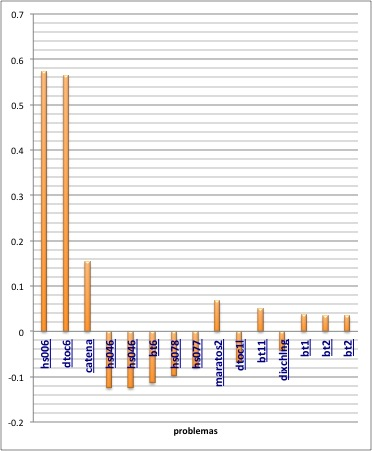
\includegraphics[trim = 0mm 0mm 00mm 0mm, clip, scale=1.2]{rendimiento(feval).jpg}\\
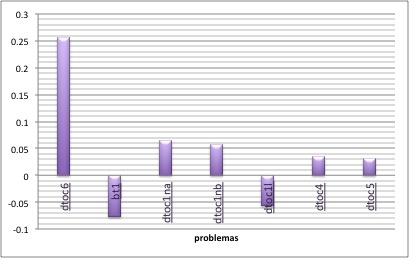
\includegraphics[trim = 0mm 0mm 10mm 0mm, scale=1.2]{rendimientos(s).jpg}\\
{\small{\noi La gr\'afica de arriba representa la comparaci\'on de los problemas que los dos algoritmos lograron resolver en t\'ermino de n\'umero de evaluaciones de la funci\'on. Como las primeras 3 barras dominan a las dem\'as en magnitud, se puede decir que el programa $PCS_{global}$ evalua m\'as veces la funci\'on que $PCS_{local}$\\
La gr\'afica de abajo representa la comparaci\'on de los problemas en t\'ermino de tiempo de ejecuci\'on. Dtoc6 es el \'unico problema que significativamente tiene una diferencia en las dos comparaciones, agregarle una penalizaci\'on a este problema no es muy efectivo en general.}}

%% Table generated by Excel2LaTeX from sheet 'Sheet1'
%\begin{table}[htbp]
%  \centering
%  \caption{byrdsphr}
%    \begin{tabular}{rrrrrr}
%    \toprule
%    k     & f     & $||c||$ & $||gL||$   & alpha & mu \\
%    \midrule
%    1     & 1.22E+01 & 2.02E+00 & 4.93E+00 & 1.25E-01 & 4.29E-01 \\
%    \bottomrule
%    \end{tabular}%
%  \label{tab:addlabel}%
%\end{table}%
%\noi Problema byrdsphr mal escalado desde el primer paso.

%% Table generated by Excel2LaTeX from sheet 'Sheet1'
%\begin{table}[htbp]
%  \centering
%  \caption{dtoc1na}
%    \begin{tabular}{rrrrrr}
%    \toprule
%    k     & f     & $||c||$ & $||gL||$   & alpha & mu \\
%    \midrule
%    1     & 1.99E+01 & 1.90E-03 & 1.48E-01 & 1.00E+00 & 4.29E-01 \\
%    2     & 1.34E+01 & 3.46E-03 & 2.69E-01 & 1.00E+00 & 4.29E-01 \\
%    3     & 1.27E+01 & 1.53E-04 & 3.27E-02 & 1.00E+00 & 4.29E-01 \\
%%    4     & 1.27E+01 & 8.09E-06 & 1.54E-03 & 1.00E+00 & 4.29E-01 \\
%%    5     & 1.27E+01 & 1.89E-08 & 3.44E-06 & 1.00E+00 & 1.29E+01 \\
%%    6     & 1.27E+01 & 8.75E-14 & 1.72E-11 & 1.00E+00 & 1.29E+01 \\
%%    7     & 1.27E+01 & 2.22E-16 & 6.67E-16 & 1.00E+00 & 1.29E+01 \\
%%    8     & 1.27E+01 & 2.22E-16 & 5.05E-16 & 5.00E-01 & 1.29E+01 \\
%%    9     & 1.27E+01 & 2.22E-16 & 5.10E-16 & 1.25E-01 & 1.29E+01 \\
%%    10    & 1.27E+01 & 2.22E-16 & 4.65E-16 & 5.00E-01 & 1.29E+01 \\
%%    11    & 1.27E+01 & 1.94E-16 & 4.30E-16 & 2.50E-01 & 1.29E+01 \\
%%    12    & 1.27E+01 & 1.94E-16 & 4.49E-16 & 2.50E-01 & 1.29E+01 \\
%%    13    & 1.27E+01 & 1.94E-16 & 4.72E-16 & 1.25E-01 & 1.29E+01 \\
%%    14    & 1.27E+01 & 1.94E-16 & 4.30E-16 & 1.25E-01 & 1.29E+01 \\
%%    15    & 1.27E+01 & 1.94E-16 & 4.44E-16 & 6.25E-02 & 1.29E+01 \\
%%    16    & 1.27E+01 & 1.94E-16 & 4.74E-16 & 1.25E-01 & 1.29E+01 \\
%%    17    & 1.27E+01 & 1.94E-16 & 4.83E-16 & 2.50E-01 & 1.29E+01 \\
%%    18    & 1.27E+01 & 1.94E-16 & 4.81E-16 & 1.25E-01 & 1.29E+01 \\
%%    19    & 1.27E+01 & 1.94E-16 & 4.58E-16 & 6.25E-02 & 1.29E+01 \\
%%    20    & 1.27E+01 & 1.94E-16 & 4.44E-16 & 2.50E-01 & 1.29E+01 \\
%%    21    & 1.27E+01 & 1.94E-16 & 4.03E-16 & 1.25E-01 & 1.29E+01 \\
%%    22    & 1.27E+01 & 1.94E-16 & 3.72E-16 & 1.25E-01 & 1.29E+01 \\
%%    23    & 1.27E+01 & 1.94E-16 & 3.68E-16 & 6.25E-02 & 1.29E+01 \\
%%    24    & 1.27E+01 & 1.94E-16 & 3.96E-16 & 6.25E-02 & 1.29E+01 \\
%%    25    & 1.27E+01 & 1.94E-16 & 3.75E-16 & 1.25E-01 & 1.29E+01 \\
%%    26    & 1.27E+01 & 1.94E-16 & 3.66E-16 & 1.25E-01 & 1.29E+01 \\
%%    27    & 1.27E+01 & 1.94E-16 & 3.81E-16 & 1.25E-01 & 1.29E+01 \\
%%    28    & 1.27E+01 & 1.94E-16 & 3.68E-16 & 6.25E-02 & 1.29E+01 \\
%%    29    & 1.27E+01 & 2.01E-16 & 3.68E-16 & 2.50E-01 & 1.29E+01 \\
%%    30    & 1.27E+01 & 2.01E-16 & 4.05E-16 & 1.25E-01 & 1.29E+01 \\
%%    31    & 1.27E+01 & 2.01E-16 & 3.65E-16 & 1.25E-01 & 1.29E+01 \\
%%    32    & 1.27E+01 & 2.01E-16 & 3.79E-16 & 1.25E-01 & 1.29E+01 \\
%%    33    & 1.27E+01 & 2.01E-16 & 3.78E-16 & 6.25E-02 & 1.29E+01 \\
%%    34    & 1.27E+01 & 1.94E-16 & 3.66E-16 & 1.25E-01 & 1.29E+01 \\
%%    35    & 1.27E+01 & 1.94E-16 & 3.96E-16 & 1.25E-01 & 1.29E+01 \\
%%    36    & 1.27E+01 & 1.94E-16 & 3.68E-16 & 6.25E-02 & 1.29E+01 \\
%%    37    & 1.27E+01 & 1.67E-16 & 4.09E-16 & 5.00E-01 & 1.29E+01 \\
%%    38    & 1.27E+01 & 1.67E-16 & 3.68E-16 & 1.25E-01 & 1.29E+01 \\
%%    39    & 1.27E+01 & 1.67E-16 & 3.89E-16 & 1.25E-01 & 1.29E+01 \\
%%    40    & 1.27E+01 & 1.67E-16 & 4.02E-16 & 1.25E-01 & 1.29E+01 \\
%%    41    & 1.27E+01 & 1.67E-16 & 3.55E-16 & 1.25E-01 & 1.29E+01 \\
%%    42    & 1.27E+01 & 1.11E-16 & 3.75E-16 & 2.50E-01 & 1.29E+01 \\
%%    43    & 1.27E+01 & 1.11E-16 & 3.78E-16 & 1.25E-01 & 1.29E+01 \\
%%    44    & 1.27E+01 & 1.11E-16 & 3.68E-16 & 1.25E-01 & 1.29E+01 \\
%%    45    & 1.27E+01 & 1.11E-16 & 4.02E-16 & 1.25E-01 & 1.29E+01 \\
%%    46    & 1.27E+01 & 1.11E-16 & 4.09E-16 & 1.25E-01 & 1.29E+01 \\
%%    47    & 1.27E+01 & 1.11E-16 & 4.23E-16 & 1.25E-01 & 1.29E+01 \\
%%    48    & 1.27E+01 & 1.11E-16 & 4.09E-16 & 1.25E-01 & 1.29E+01 \\
%%    49    & 1.27E+01 & 1.11E-16 & 4.16E-16 & 1.25E-01 & 1.29E+01 \\
%%    50    & 1.27E+01 & 1.67E-16 & 4.16E-16 & 2.50E-01 & 1.29E+01 \\
%%    51    & 1.27E+01 & 1.67E-16 & 3.98E-16 & 1.25E-01 & 1.29E+01 \\
%%    52    & 1.27E+01 & 1.67E-16 & 3.84E-16 & 2.50E-01 & 1.29E+01 \\
%%    53    & 1.27E+01 & 1.67E-16 & 4.05E-16 & 2.50E-01 & 1.29E+01 \\
%%    54    & 1.27E+01 & 1.67E-16 & 4.15E-16 & 1.25E-01 & 1.29E+01 \\
%%    55    & 1.27E+01 & 1.67E-16 & 4.42E-16 & 1.25E-01 & 1.29E+01 \\
%%    56    & 1.27E+01 & 1.67E-16 & 4.44E-16 & 6.25E-02 & 1.29E+01 \\
%%    57    & 1.27E+01 & 1.67E-16 & 4.22E-16 & 1.25E-01 & 1.29E+01 \\
%%    58    & 1.27E+01 & 1.67E-16 & 4.40E-16 & 1.25E-01 & 1.29E+01 \\
%%    59    & 1.27E+01 & 1.67E-16 & 4.26E-16 & 1.25E-01 & 1.29E+01 \\
%%    60    & 1.27E+01 & 1.67E-16 & 4.14E-16 & 1.25E-01 & 1.29E+01 \\
%%    61    & 1.27E+01 & 1.67E-16 & 4.65E-16 & 2.50E-01 & 1.29E+01 \\
%%    62    & 1.27E+01 & 1.67E-16 & 4.55E-16 & 1.25E-01 & 1.29E+01 \\
%%    63    & 1.27E+01 & 1.67E-16 & 4.26E-16 & 1.25E-01 & 1.29E+01 \\
%%    64    & 1.27E+01 & 1.67E-16 & 4.28E-16 & 1.25E-01 & 1.29E+01 \\
%%    65    & 1.27E+01 & 1.67E-16 & 4.23E-16 & 1.25E-01 & 1.29E+01 \\
%%    66    & 1.27E+01 & 1.67E-16 & 3.99E-16 & 1.25E-01 & 1.29E+01 \\
%%    67    & 1.27E+01 & 1.67E-16 & 3.88E-16 & 1.25E-01 & 1.29E+01 \\
%%    68    & 1.27E+01 & 2.01E-16 & 4.72E-16 & 2.50E-01 & 1.29E+01 \\
%%    69    & 1.27E+01 & 2.01E-16 & 4.65E-16 & 6.25E-02 & 1.29E+01 \\
%%    70    & 1.27E+01 & 2.01E-16 & 4.65E-16 & 1.25E-01 & 1.29E+01 \\
%%    71    & 1.27E+01 & 2.01E-16 & 4.44E-16 & 6.25E-02 & 1.29E+01 \\
%%    72    & 1.27E+01 & 2.01E-16 & 4.23E-16 & 6.25E-02 & 1.29E+01 \\
%%    73    & 1.27E+01 & 2.01E-16 & 4.51E-16 & 6.25E-02 & 1.29E+01 \\
%%    74    & 1.27E+01 & 2.01E-16 & 4.51E-16 & 6.25E-02 & 1.29E+01 \\
%%    75    & 1.27E+01 & 2.01E-16 & 4.23E-16 & 6.25E-02 & 1.29E+01 \\
%%    76    & 1.27E+01 & 2.01E-16 & 4.26E-16 & 1.25E-01 & 1.29E+01 \\
%%    77    & 1.27E+01 & 2.01E-16 & 4.25E-16 & 6.25E-02 & 1.29E+01 \\
%%    78    & 1.27E+01 & 2.01E-16 & 4.17E-16 & 1.25E-01 & 1.29E+01 \\
%%    79    & 1.27E+01 & 2.01E-16 & 4.23E-16 & 6.25E-02 & 1.29E+01 \\
%%    80    & 1.27E+01 & 2.01E-16 & 4.27E-16 & 6.25E-02 & 1.29E+01 \\
%%    81    & 1.27E+01 & 2.01E-16 & 4.20E-16 & 6.25E-02 & 1.29E+01 \\
%%    82    & 1.27E+01 & 2.01E-16 & 4.22E-16 & 6.25E-02 & 1.29E+01 \\
%%    83    & 1.27E+01 & 2.01E-16 & 4.25E-16 & 1.25E-01 & 1.29E+01 \\
%%    84    & 1.27E+01 & 2.01E-16 & 4.33E-16 & 1.25E-01 & 1.29E+01 \\
%%    85    & 1.27E+01 & 2.01E-16 & 4.20E-16 & 6.25E-02 & 1.29E+01 \\
%%    86    & 1.27E+01 & 2.01E-16 & 4.24E-16 & 6.25E-02 & 1.29E+01 \\
%%    87    & 1.27E+01 & 2.01E-16 & 4.24E-16 & 1.25E-01 & 1.29E+01 \\
%%    88    & 1.27E+01 & 2.01E-16 & 3.96E-16 & 1.25E-01 & 1.29E+01 \\
%%    89    & 1.27E+01 & 2.01E-16 & 4.09E-16 & 6.25E-02 & 1.29E+01 \\
%    90    & 1.27E+01 & 2.01E-16 & 3.86E-16 & 6.25E-02 & 1.29E+01 \\
%    91    & 1.27E+01 & 2.01E-16 & 4.00E-16 & 6.25E-02 & 1.29E+01 \\
%    92    & 1.27E+01 & 2.01E-16 & 4.01E-16 & 6.25E-02 & 1.29E+01 \\
%    93    & 1.27E+01 & 2.01E-16 & 3.95E-16 & 6.25E-02 & 1.29E+01 \\
%    94    & 1.27E+01 & 2.01E-16 & 3.95E-16 & 6.25E-02 & 1.29E+01 \\
%    95    & 1.27E+01 & 2.01E-16 & 3.95E-16 & 6.25E-02 & 1.29E+01 \\
%    96    & 1.27E+01 & 2.01E-16 & 3.96E-16 & 1.25E-01 & 1.29E+01 \\
%    97    & 1.27E+01 & 2.01E-16 & 4.23E-16 & 1.25E-01 & 1.29E+01 \\
%    98    & 1.27E+01 & 2.01E-16 & 4.16E-16 & 1.25E-01 & 1.29E+01 \\
%    99    & 1.27E+01 & 2.01E-16 & 3.61E-16 & 2.50E-01 & 1.29E+01 \\
%    100   & 1.27E+01 & 2.01E-16 & 3.61E-16 & 6.25E-02 & 1.29E+01 \\
%    101   & 1.27E+01 & 2.01E-16 & 4.09E-16 & 1.25E-01 & 1.29E+01 \\
%    \bottomrule
%    \end{tabular}%
%  \label{tab:addlabel}%
%\end{table}%
%\noi Aqu\'i se puede ver que el problema dtoc1na parec\'ia ya haber convergido pero sigui\'o iterando hasta pasar maxiter dadas las condiciones de paro.
% 
% 
%\pagebreak
%
%% Table generated by Excel2LaTeX from sheet 'Sheet1'
%\begin{table}[htbp]
%  \centering
%  \caption{dtoc1l}
%    \begin{tabular}{rrrrrr}
%    \toprule
%    k     & f     & $||c||$ & $||gL||$   & alpha & mu \\
%    \midrule
%    1     & 2.01E+02 & 4.44E-16 & 1.47E-01 & 1.00E+00 & 4.29E-01 \\
%    2     & 1.34E+02 & 1.33E-15 & 2.92E-01 & 1.00E+00 & 4.29E-01 \\
%    3     & 1.26E+02 & 8.33E-16 & 3.67E-02 & 1.00E+00 & 4.29E-01 \\
%    4     & 1.25E+02 & 1.78E-15 & 1.86E-03 & 1.00E+00 & 4.29E-01 \\
%    5     & 1.25E+02 & 1.25E-15 & 5.03E-06 & 1.00E+00 & 4.29E-01 \\
%    6     & 1.25E+02 & 1.17E-15 & 3.61E-11 & 1.00E+00 & 4.29E-01 \\
%    7     & 1.25E+02 & 1.03E-15 & 3.16E-11 & 1.25E-01 & 6.24E+00 \\
%    8     & 1.25E+02 & 1.03E-15 & 3.16E-11 & 6.10E-05 & 2.86E+01 \\
%    9     & 1.25E+02 & 1.03E-15 & 3.16E-11 & 6.10E-05 & 2.86E+01 \\
%    10    & 1.25E+02 & 1.05E-15 & 3.16E-11 & 6.10E-05 & 2.86E+01 \\
%    11    & 1.25E+02 & 1.05E-15 & 3.16E-11 & 6.10E-05 & 2.86E+01 \\
%    12    & 1.25E+02 & 1.08E-15 & 3.16E-11 & 6.10E-05 & 2.86E+01 \\
%    13    & 1.25E+02 & 1.08E-15 & 3.16E-11 & 6.10E-05 & 2.86E+01 \\
%    14    & 1.25E+02 & 1.11E-15 & 3.16E-11 & 6.10E-05 & 2.86E+01 \\
%%    15    & 1.25E+02 & 1.11E-15 & 3.16E-11 & 6.10E-05 & 2.86E+01 \\
%%    16    & 1.25E+02 & 1.11E-15 & 3.16E-11 & 6.10E-05 & 2.86E+01 \\
%%    17    & 1.25E+02 & 1.11E-15 & 3.16E-11 & 3.05E-05 & 2.86E+01 \\
%%    18    & 1.25E+02 & 1.11E-15 & 3.16E-11 & 7.63E-06 & 2.86E+01 \\
%%    19    & 1.25E+02 & 1.11E-15 & 3.16E-11 & 1.91E-06 & 2.86E+01 \\
%%    20    & 1.25E+02 & 1.11E-15 & 3.16E-11 & 1.91E-06 & 2.86E+01 \\
%%    21    & 1.25E+02 & 1.11E-15 & 3.16E-11 & 1.91E-06 & 2.86E+01 \\
%%    22    & 1.25E+02 & 1.11E-15 & 3.16E-11 & 1.91E-06 & 2.86E+01 \\
%%    23    & 1.25E+02 & 1.11E-15 & 3.16E-11 & 1.91E-06 & 2.86E+01 \\
%%    24    & 1.25E+02 & 1.11E-15 & 3.16E-11 & 1.91E-06 & 2.86E+01 \\
%%    25    & 1.25E+02 & 1.11E-15 & 3.16E-11 & 1.91E-06 & 2.86E+01 \\
%%    26    & 1.25E+02 & 1.11E-15 & 3.16E-11 & 1.91E-06 & 2.86E+01 \\
%%    27    & 1.25E+02 & 1.11E-15 & 3.16E-11 & 1.91E-06 & 2.86E+01 \\
%%    28    & 1.25E+02 & 1.11E-15 & 3.16E-11 & 1.91E-06 & 2.86E+01 \\
%%    29    & 1.25E+02 & 1.11E-15 & 3.16E-11 & 1.91E-06 & 2.86E+01 \\
%%    30    & 1.25E+02 & 1.11E-15 & 3.16E-11 & 1.91E-06 & 2.86E+01 \\
%%    31    & 1.25E+02 & 1.11E-15 & 3.16E-11 & 1.91E-06 & 2.86E+01 \\
%%    32    & 1.25E+02 & 1.11E-15 & 3.16E-11 & 1.91E-06 & 2.86E+01 \\
%%    33    & 1.25E+02 & 1.11E-15 & 3.16E-11 & 1.91E-06 & 2.86E+01 \\
%%    34    & 1.25E+02 & 1.11E-15 & 3.16E-11 & 1.91E-06 & 2.86E+01 \\
%%    35    & 1.25E+02 & 1.11E-15 & 3.16E-11 & 1.91E-06 & 2.86E+01 \\
%%    36    & 1.25E+02 & 1.11E-15 & 3.16E-11 & 1.91E-06 & 2.86E+01 \\
%    37    & 1.25E+02 & 1.11E-15 & 3.16E-11 & 1.91E-06 & 2.86E+01 \\
%    38    & 1.25E+02 & 1.11E-15 & 3.16E-11 & 1.91E-06 & 2.86E+01 \\
%    39    & 1.25E+02 & 1.17E-15 & 3.16E-11 & 1.91E-06 & 2.86E+01 \\
%    40    & 1.25E+02 & 1.22E-15 & 3.16E-11 & 1.91E-06 & 2.86E+01 \\
%    \bottomrule
%    \end{tabular}%
%  \label{tab:addlabel}%
%\end{table}%
%% Table generated by Excel2LaTeX from sheet 'Sheet1'
%\begin{table}[htbp]
%  \centering
%  \caption{hs046}
%    \begin{tabular}{rrrrrr}
%    \toprule
%    k     & f     & $||c||$ & $||gL||$   & alpha & mu \\
%    \midrule
%    1     & 7.04E-01 & 4.80E+00 & 1.73E+01 & 1.00E+00 & 5.33E-01 \\
%    2     & 3.73E-01 & 1.23E+00 & 5.09E+00 & 1.00E+00 & 5.33E-01 \\
%    3     & 8.33E-02 & 2.71E-01 & 1.39E+00 & 1.00E+00 & 5.33E-01 \\
%    4     & 2.03E-02 & 3.35E-02 & 2.63E-01 & 1.00E+00 & 5.33E-01 \\
%%    5     & 5.72E-03 & 9.59E-03 & 5.54E-02 & 1.00E+00 & 5.33E-01 \\
%%    6     & 1.14E-03 & 9.95E-03 & 1.69E-02 & 1.00E+00 & 5.33E-01 \\
%%    7     & 1.06E-06 & 4.61E-03 & 1.20E-03 & 1.00E+00 & 5.33E-01 \\
%%    8     & 4.57E-08 & 4.22E-06 & 3.38E-05 & 1.00E+00 & 5.33E-01 \\
%%    9     & 3.24E-08 & 3.19E-06 & 2.56E-05 & 2.50E-01 & 5.33E-01 \\
%%    10    & 2.30E-08 & 2.42E-06 & 1.94E-05 & 2.50E-01 & 5.33E-01 \\
%%    11    & 1.63E-08 & 1.83E-06 & 1.47E-05 & 2.50E-01 & 5.33E-01 \\
%%    12    & 1.37E-08 & 1.69E-06 & 1.29E-05 & 1.25E-01 & 5.33E-01 \\
%%    13    & 1.16E-08 & 1.67E-06 & 1.13E-05 & 1.25E-01 & 5.33E-01 \\
%%    14    & 9.81E-09 & 1.65E-06 & 9.91E-06 & 1.25E-01 & 5.33E-01 \\
%%    15    & 8.28E-09 & 1.61E-06 & 8.69E-06 & 1.25E-01 & 5.33E-01 \\
%%    16    & 6.99E-09 & 1.56E-06 & 7.62E-06 & 1.25E-01 & 5.33E-01 \\
%%    17    & 5.91E-09 & 1.51E-06 & 6.69E-06 & 1.25E-01 & 5.33E-01 \\
%%    18    & 4.99E-09 & 1.45E-06 & 5.86E-06 & 1.25E-01 & 5.33E-01 \\
%%    19    & 4.21E-09 & 1.39E-06 & 5.14E-06 & 1.25E-01 & 5.33E-01 \\
%%    20    & 3.55E-09 & 1.32E-06 & 4.51E-06 & 1.25E-01 & 5.33E-01 \\
%%    21    & 3.00E-09 & 1.26E-06 & 3.96E-06 & 1.25E-01 & 5.33E-01 \\
%%    22    & 2.53E-09 & 1.20E-06 & 3.47E-06 & 1.25E-01 & 5.33E-01 \\
%%    23    & 2.14E-09 & 1.13E-06 & 3.04E-06 & 1.25E-01 & 5.33E-01 \\
%%    24    & 1.80E-09 & 1.07E-06 & 2.67E-06 & 1.25E-01 & 5.33E-01 \\
%%    25    & 1.52E-09 & 1.01E-06 & 2.34E-06 & 1.25E-01 & 5.33E-01 \\
%%    26    & 1.29E-09 & 9.50E-07 & 2.05E-06 & 1.25E-01 & 5.33E-01 \\
%%    27    & 1.08E-09 & 8.93E-07 & 1.80E-06 & 1.25E-01 & 5.33E-01 \\
%%    28    & 9.15E-10 & 8.38E-07 & 1.58E-06 & 1.25E-01 & 5.33E-01 \\
%%    29    & 6.47E-10 & 8.36E-07 & 1.20E-06 & 2.50E-01 & 5.33E-01 \\
%%    30    & 4.57E-10 & 8.02E-07 & 9.09E-07 & 2.50E-01 & 5.33E-01 \\
%%    31    & 3.23E-10 & 7.49E-07 & 6.90E-07 & 2.50E-01 & 5.33E-01 \\
%%    32    & 2.28E-10 & 6.86E-07 & 5.24E-07 & 2.50E-01 & 5.33E-01 \\
%%    33    & 1.61E-10 & 6.19E-07 & 3.97E-07 & 2.50E-01 & 5.33E-01 \\
%%    34    & 1.14E-10 & 5.52E-07 & 3.02E-07 & 2.50E-01 & 5.33E-01 \\
%%    35    & 8.05E-11 & 4.88E-07 & 2.29E-07 & 2.50E-01 & 5.33E-01 \\
%%    36    & 5.69E-11 & 4.28E-07 & 1.74E-07 & 2.50E-01 & 5.33E-01 \\
%%    37    & 2.74E-11 & 4.23E-07 & 9.35E-08 & 5.00E-01 & 5.33E-01 \\
%%    38    & 1.32E-11 & 3.57E-07 & 5.05E-08 & 5.00E-01 & 5.33E-01 \\
%%    39    & 6.39E-12 & 2.79E-07 & 2.74E-08 & 5.00E-01 & 5.33E-01 \\
%%    40    & 3.08E-12 & 2.10E-07 & 1.50E-08 & 5.00E-01 & 5.33E-01 \\
%%    41    & 6.09E-13 & 1.95E-07 & 2.76E-09 & 1.00E+00 & 5.33E-01 \\
%%    42    & 1.20E-13 & 8.67E-08 & 8.17E-10 & 1.00E+00 & 5.33E-01 \\
%%    43    & 2.38E-14 & 3.85E-08 & 2.42E-10 & 1.00E+00 & 5.33E-01 \\
%%    44    & 4.70E-15 & 1.71E-08 & 7.17E-11 & 1.00E+00 & 5.33E-01 \\
%%    45    & 9.27E-16 & 7.61E-09 & 2.13E-11 & 1.00E+00 & 5.33E-01 \\
%%    46    & 1.83E-16 & 3.38E-09 & 6.30E-12 & 1.00E+00 & 5.33E-01 \\
%%    47    & 3.62E-17 & 1.50E-09 & 1.87E-12 & 1.00E+00 & 5.33E-01 \\
%%    48    & 7.15E-18 & 6.68E-10 & 5.53E-13 & 1.00E+00 & 5.33E-01 \\
%%    49    & 1.41E-18 & 2.97E-10 & 1.64E-13 & 1.00E+00 & 5.33E-01 \\
%%    50    & 2.79E-19 & 1.32E-10 & 4.85E-14 & 1.00E+00 & 5.33E-01 \\
%%    51    & 5.51E-20 & 5.87E-11 & 1.44E-14 & 1.00E+00 & 5.33E-01 \\
%%    52    & 1.09E-20 & 2.61E-11 & 4.26E-15 & 1.00E+00 & 5.33E-01 \\
%%    53    & 2.15E-21 & 1.16E-11 & 1.26E-15 & 1.00E+00 & 5.33E-01 \\
%%    54    & 4.25E-22 & 5.15E-12 & 3.74E-16 & 1.00E+00 & 5.33E-01 \\
%    55    & 8.39E-23 & 2.29E-12 & 1.11E-16 & 1.00E+00 & 5.33E-01 \\
%    56    & 1.66E-23 & 1.02E-12 & 3.28E-17 & 1.00E+00 & 5.33E-01 \\
%    57    & 3.27E-24 & 4.52E-13 & 9.73E-18 & 1.00E+00 & 5.33E-01 \\
%    58    & 6.46E-25 & 2.02E-13 & 2.88E-18 & 1.00E+00 & 5.33E-01 \\
%    59    & 1.28E-25 & 8.93E-14 & 8.54E-19 & 1.00E+00 & 5.33E-01 \\
%    60    & 2.52E-26 & 3.95E-14 & 2.53E-19 & 1.00E+00 & 5.33E-01 \\
%    61    & 4.98E-27 & 1.78E-14 & 7.50E-20 & 1.00E+00 & 5.33E-01 \\
%    62    & 9.84E-28 & 7.99E-15 & 2.22E-20 & 1.00E+00 & 5.33E-01 \\
%    63    & 1.94E-28 & 3.55E-15 & 6.59E-21 & 1.00E+00 & 5.33E-01 \\
%    64    & 3.84E-29 & 8.88E-16 & 1.95E-21 & 1.00E+00 & 5.33E-01 \\
%    65    & 1.85E-29 & 4.44E-16 & 1.13E-21 & 5.00E-01 & 5.33E-01 \\
%    \bottomrule
%    \end{tabular}%
%  \label{tab:addlabel}%
%\end{table} $$$$
%En el caso de dtoc1l y hs046, se puede notar que, desde varias iteraciones antes, el problema ten\'ia normas suficientemente peque\~nas como para terminar pero no paraba dado que (probablemente) la norma en el c\'alculo inicial de las restricciones y del gradiente de la funci\'on lagrangiana ya eran demasiado peque\~nas para alcanzarlas (TOL = 10e-7). 
%
%\pagebreak
%% Table generated by Excel2LaTeX from sheet 'Sheet1'
%\begin{table}[htbp]
%  \centering
%  \caption{orthregc}
%    \begin{tabular}{rrrrrr}
%    \toprule
%    k     & f     & $||c||$ & $||gL||$   & alpha & mu \\
%    \midrule
%    1     & 1.54E+01 & 3.86E+00 & 4.75E+01 & 5.00E-01 & 9.01E+00 \\
%    2     & 1.91E+02 & 1.87E+00 & 1.83E+03 & 5.00E-01 & 1.75E+02 \\
%    \bottomrule
%    \end{tabular}%
%  \label{tab:addlabel}%
%\end{table}%
%\noi orthregc es el ejemplo de un caso en donde la matriz tiene una inercia incorrecta, se puede ver que, en lugar de impulsar un verdadero descenso, lo ganado en las restricciones (asegurar factibilidad) se pierde en la funci\'on objetivo. Esta p\'erdida probablemente sea impulsada por el valor alto de $\mu$ ($\mu = 9.01$) que carga el peso de la funci\'on de m\'erito sobre la norma de las restricciones.
% % Table generated by Excel2LaTeX from sheet 'Sheet1'
%\begin{table}[htbp]
%  \centering
%  \caption{dtoc5}
%    \begin{tabular}{rrrrrr}
%    \toprule
%    k     & f     & $||c||$ & $||gL||$   & alpha & mu \\
%    \midrule
%    1     & 7.62E-01 & 2.00E-04 & 6.09E-04 & 1.00E+00 & 8.46E-01 \\
%    2     & 1.53E+00 & 1.58E-05 & 1.70E-05 & 1.00E+00 & 4.29E+03 \\
%    3     & 1.54E+00 & 6.90E-09 & 2.50E-08 & 1.00E+00 & 4.29E+03 \\
%    \bottomrule
%    \end{tabular}%
%  \label{tab:addlabel}%
%\end{table}%
%
%% Table generated by Excel2LaTeX from sheet 'Sheet1'
%\begin{table}[htbp]
%  \centering
%  \caption{dtoc4}
%    \begin{tabular}{rrrrrr}
%    \toprule
%    k     & f     & $||c||$ & $||gL||$   & alpha & mu \\
%    \midrule
%    1     & 3.37E+00 & 3.39E-04 & 1.74E-03 & 1.00E+00 & 3.75E+00 \\
%    2     & 2.87E+00 & 3.15E-07 & 1.48E-05 & 1.00E+00 & 3.75E+00 \\
%    3     & 2.87E+00 & 1.59E-10 & 1.02E-09 & 1.00E+00 & 3.39E+02 \\
%    \bottomrule
%    \end{tabular}%
%  \label{tab:addlabel}%
%\end{table}%
%\noi Sin embargo, hay casos como dtoc4 y dtoc5 que sin importar el gran n\'umero de variables y restricciones, alcanzan su m\'inimo en pocas iteraciones. De hecho, la alfa se mantiene "inactiva" durante todo el proceso, indicando que no necesitan ning\'un corte los avances dados por el programa.
% \pagebreak
%
%
%% Table generated by Excel2LaTeX from sheet 'Sheet1'
%\begin{table}[htbp]
%  \centering
%  \caption{dtoc6}
%    \begin{tabular}{rrrrrr}
%    \toprule
%    k     & f     & $||c||$ & $||gL||$   & alpha & mu \\
%    \midrule
%    1     & 1.54E+03 & 6.16E-01 & 6.07E-01 & 5.00E-01 & 1.00E+00 \\
%    2     & 2.84E+03 & 3.71E-01 & 3.69E-01 & 5.00E-01 & 9.02E+03 \\
%    3     & 5.75E+03 & 2.26E-01 & 4.63E-01 & 5.00E-01 & 2.67E+04 \\
%    4     & 1.00E+04 & 1.40E-01 & 6.09E-01 & 5.00E-01 & 6.12E+04 \\
%    5     & 1.56E+04 & 8.54E-02 & 7.45E-01 & 5.00E-01 & 1.26E+05 \\
%    6     & 2.25E+04 & 5.16E-02 & 8.73E-01 & 5.00E-01 & 2.51E+05 \\
%    7     & 3.05E+04 & 3.12E-02 & 9.97E-01 & 5.00E-01 & 4.87E+05 \\
%    8     & 3.98E+04 & 1.88E-02 & 1.12E+00 & 5.00E-01 & 9.23E+05 \\
%    9     & 5.02E+04 & 1.14E-02 & 1.24E+00 & 5.00E-01 & 1.71E+06 \\
%    10    & 6.17E+04 & 6.86E-03 & 1.35E+00 & 5.00E-01 & 3.11E+06 \\
%    11    & 7.41E+04 & 4.15E-03 & 1.47E+00 & 5.00E-01 & 5.50E+06 \\
%    12    & 8.70E+04 & 2.51E-03 & 1.58E+00 & 5.00E-01 & 9.40E+06 \\
%    13    & 1.00E+05 & 1.51E-03 & 1.66E+00 & 5.00E-01 & 1.52E+07 \\
%    14    & 1.12E+05 & 8.57E-04 & 1.52E+00 & 5.00E-01 & 2.22E+07 \\
%    15    & 1.21E+05 & 5.12E-04 & 1.07E+00 & 5.00E-01 & 2.84E+07 \\
%    16    & 1.24E+05 & 4.03E-04 & 8.23E-01 & 2.50E-01 & 2.89E+07 \\
%    17    & 1.27E+05 & 3.14E-04 & 6.29E-01 & 2.50E-01 & 2.89E+07 \\
%    18    & 1.29E+05 & 2.43E-04 & 4.79E-01 & 2.50E-01 & 2.89E+07 \\
%    19    & 1.32E+05 & 1.39E-04 & 2.54E-01 & 5.00E-01 & 2.89E+07 \\
%    20    & 1.35E+05 & 1.91E-05 & 1.42E-02 & 1.00E+00 & 2.89E+07 \\
%    21    & 1.35E+05 & 5.07E-09 & 7.86E-06 & 1.00E+00 & 2.89E+07 \\
%   22    & 1.35E+05 & 4.78E-12 & 3.68E-12 & 1.00E+00 & 2.89E+07 \\
%    \bottomrule
%    \end{tabular}%
%  \label{tab:addlabel}%
%\end{table}%
% \noi En casos como en dtoc6 se puede notar que al principio el m\'etodo avanza de manera lenta (lo que ocasiona que se llegue a tantas iteraciones), sin embargo, cerca de la soluci\'on el m\'etodo acelera y converge de forma mayor a lineal, conforme esto pasa, la $\alpha$ se va volviendo menos restrictiva y deja que los pasos que da el programa sean m\'as grandes. Al mismo tiempo se puede notar que la $\mu$ cada vez va cargando m\'as el peso de la funci\'on de m\'erito sobre las restricciones, asegurando que la factibilidad no se pierda en los \'ultimos pasos con $\alpha$ cercana a 1. No existieron muchos de estos casos (m\'as de 20 iteraciones con convergencia) en los ejercicios realizados.
%
% 
%
%
%
%
%






\end{document}  